\documentclass[../design_fonctionnement_sys.tex]{subfiles}
\begin{document}

\section{Design du système}
Le système est divisé en 7 entités:
\begin{itemize}
    \item Connexion et Inscription (en rose)
    \item Gestion des comptes (en gris)
    \item Menu principal (en jaune)
    \item Profil (en bleu ciel)
    \item Matchmaking (en orange)
    \item Chat (en vert)
    \item Jeu (en bleu foncé)
    \newline
\end{itemize}

Nous allons les détailler dans différents diagrammes. A noter que toutes ces entités vont hériter des mêmes classes abstraites.
Cela est du au fait d'utiliser le design MVC pour cette application.
Chaque entité du système est donc composée de 3 composantes principales:
\begin{itemize}
    \item La vue: Elle correspond à l'interface, elle permet d'afficher les informations 
    et de reçevoir les input de l'utilisateur qu'elle communique au controller.
    \item Le controller: Il gère les requètes envoyées par la vue et les communique au serveur avec lequel il échange des informations.
    Il met le serveur à jour suite aux actions d'utilisateurs.
    \item Le serveur: il contient toutes les informations relatives aux utilisateur et à une partie. 
    Il est responsable d'envoyer les informations requise par le controller et permet de mettre les joueurs en relation pour une partie.\\
\end{itemize}

Nous utilisons également la paterne observer/subject afin que la vue soit 
automatiquement mise à jour des modifications apportée au serveur ainsi que des changement d'un menu à un autre.
Les classes vue et controller héritent donc d'une classe abstraite observer et le server d'une classe abstraite sujet.\\
En partie, chaque client est connecté au même plateau, et à son propre côté. Le game serveur fait le lien entre les deux.
Le gameController permet de mettre à jour le plateau de chaque client après une action.

\begin{figure}[H]
    \centering
    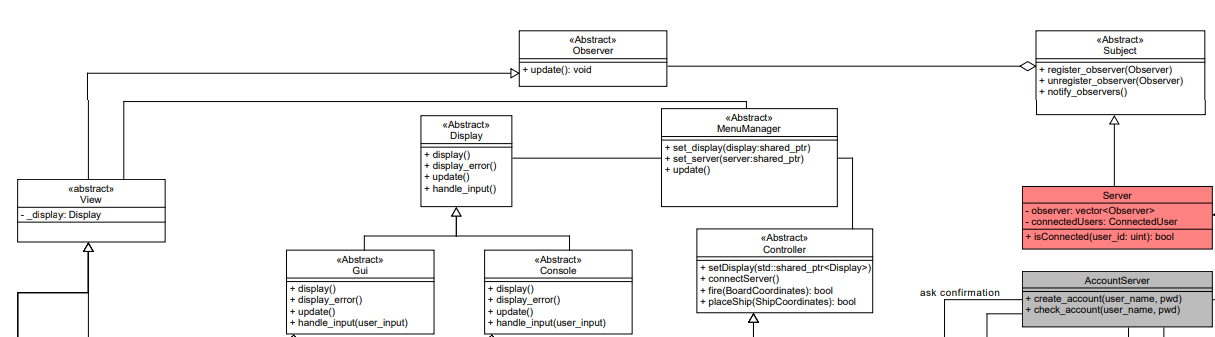
\includegraphics[scale=0.6]{img_design/Abstract.png}
    \label{fig:seq_match_server}
    \caption{Classes abstraites}
\end{figure}

\subsection{Connexion et Inscription}
Dès que le joueur lance le jeu, il a la possibilité de soit créer un compte, soit se connecter au compte qu'il a déjà. 
Il aura donc deux interfaces différentes pour ces deux actions.
\begin{figure}[H]
    \centering
    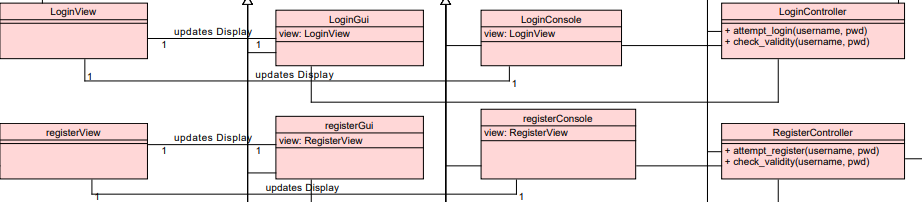
\includegraphics[scale=0.6]{img_design/Connexion_et_inscription.png}
    \label{fig:seq_match_server}
    \caption{Connexion et Inscription}
\end{figure}


\subsection{Gestion des comptes}
Le \texttt{AccountServer} permet de communiquer avec la base de donnée. Elle permet de produire des instances de la classe \texttt{Account}. 
Chaque compte a également une liste d'ami, qu'il peut gérer.

\begin{figure}[H]
    \centering
    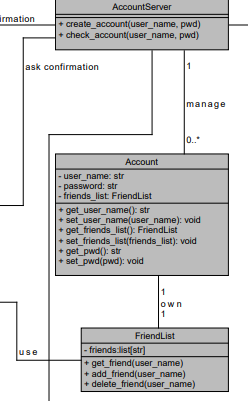
\includegraphics[scale=0.6]{img_design/Gestion_de_comptes.png}
    \label{fig:seq_match_server}
    \caption{Gestion des comptes}
\end{figure}


\subsection{Menu principal}
Le menu principal est celui qui permettra d'accéder aux autres écrans du jeu, tels que la création de partie, ou la modification de profil.
\begin{figure}[H]
    \centering
    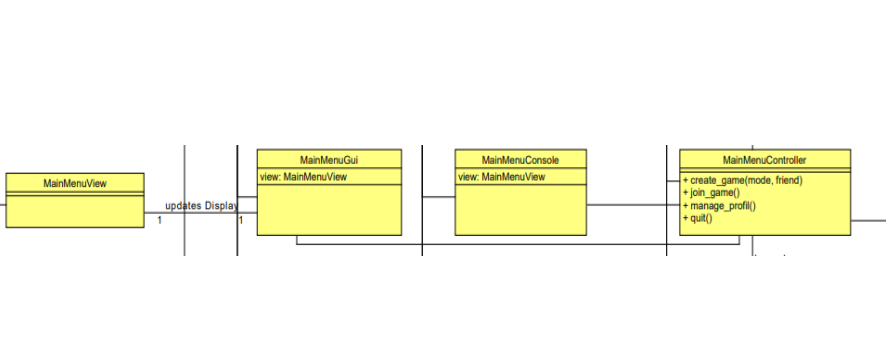
\includegraphics[scale=0.6]{img_design/Main_menu.png}
    \label{fig:seq_match_server}
    \caption{Menu principal}
\end{figure}

\subsection{Profil}
Le joueur a accès à une interface qui lui permet de modifier les informations relatives à son compte.
\begin{figure}[H]
    \centering
    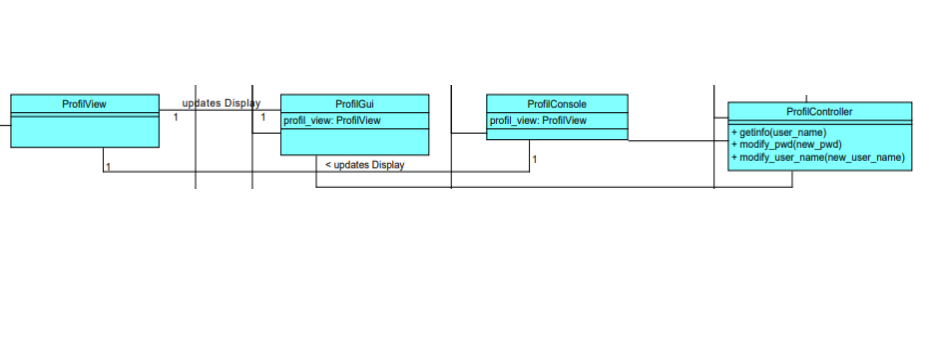
\includegraphics[scale=0.6]{img_design/Profil.png}
    \label{fig:seq_match_server}
    \caption{Profil}
\end{figure}

\subsection{Matchmaking}
La classe \texttt{MatchMaker} à une liste d'instances de \texttt{PendingMatch}, 
qui est une partie qui attend d'être lancée, car elle ne contient pas assez de joueurs.
\begin{figure}[H]
    \centering
    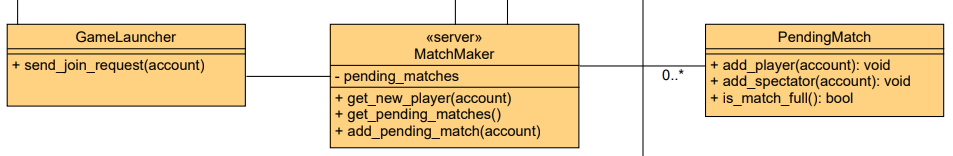
\includegraphics[scale=0.6]{img_design/Matchmaking.png}
    \label{fig:seq_match_server}
    \caption{Matchmaking}
\end{figure}

\subsection{Chat}
Le jeu offre aux joueurs un chat qui leur permet d'envoyer une chaine de caractère qui sera envoyée à tous les autres joueurs. 
Toute cette redirection de chaines de message se fait dans le \texttt{ChatServer}.
De plus, le joueur a une liste d'ami, qui affiche tous ses amis, qu'ils soient connectés ou non.
\begin{figure}[H]
    \centering
    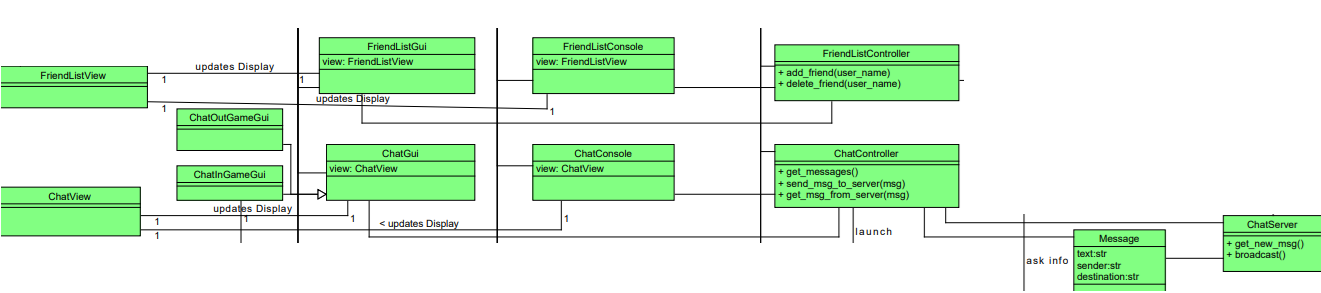
\includegraphics[scale=0.6]{img_design/Chat.png}
    \label{fig:seq_match_server}
    \caption{Chat}
\end{figure}

\subsection{Jeu}
La partie locale du jeu est concue de la manière suivante: 
le joueur a une board local qui est une copie du board du serveur (avec les cases de l'adversaire qui sont masquées), 
un controlleur qui permet de communiquer avec le serveur et un display qui permet d'afficher une partie à l'écran.
\begin{figure}[H]
    \centering
    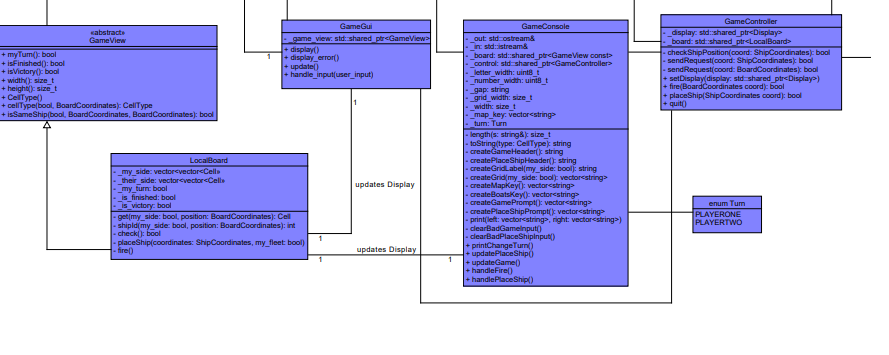
\includegraphics[scale=0.6]{img_design/Game_client.png}
    \label{fig:seq_match_server}
    \caption{Game affichage}
\end{figure}

En ce qui concerne la partie serveur d'une partie, nous avons une instance de Board qui contient les plateaux des deux joueurs, 
ainsi qu'une flotte qui appartient à ces deux joueurs. Le GameServeur est la classe qui s'occupe de la communication entre le Board et les joueurs.
\begin{figure}[H]
    \centering
    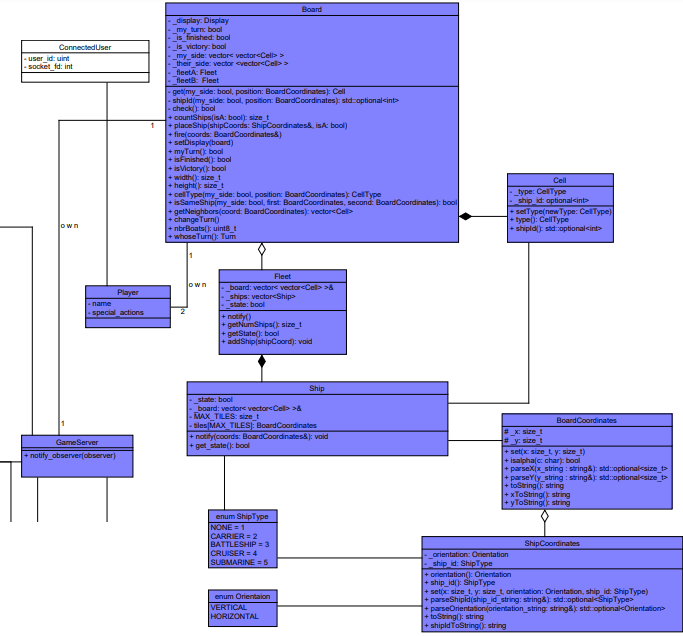
\includegraphics[scale=0.6]{img_design/Game_serveur.png}
    \label{fig:seq_match_server}
    \caption{Game serveur}
\end{figure}

\subsection{Vue globale}
Pour aider à visualiser l'interraction entre les différents acteurs et avoir une vue globale. Nous avons fait un diagramme de classe
qui reprend l'idée générale du système.
\newpage
\begin{figure}[H]
    \centering
    \rotatebox{90}{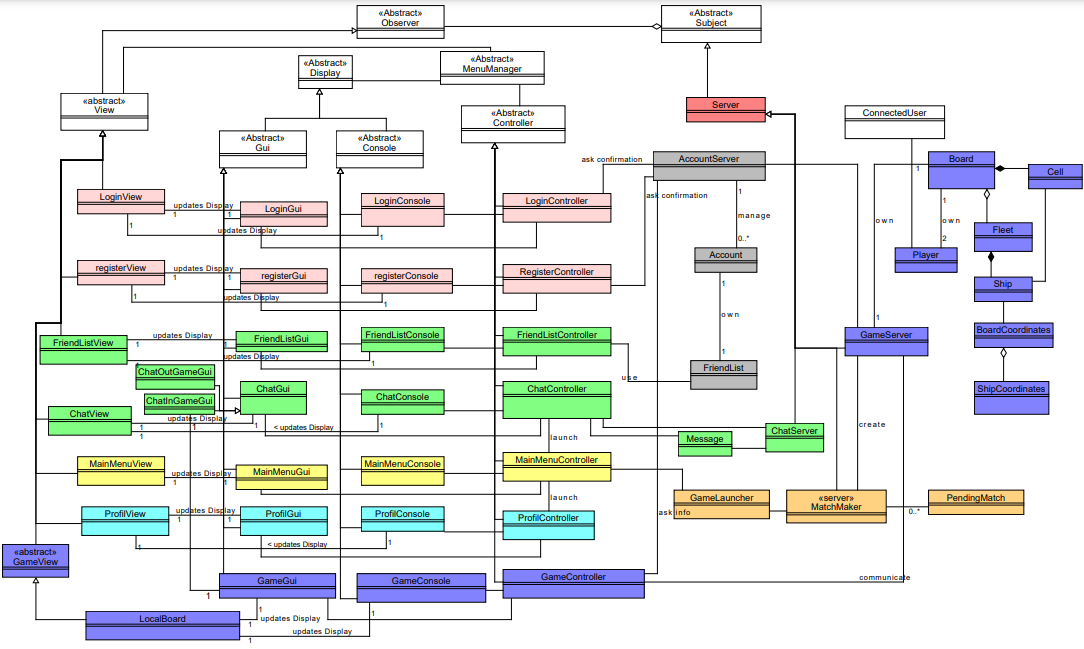
\includegraphics[scale=1]{img_design/dia_class.png}}
    \label{fig:dia_class}
    \caption{Diagramme de classe}
\end{figure}
\end{document}
